\documentclass[main]{subfiles}

\begin{document}

\chapter{Filtro de Kalman}

Con el objetivo de agregar robustez a las medidas arrojadas por los sensores, se debe implementar algún algoritmo de estimación de estados que, corriendo en tiempo real, mantenga una estimación del estado mejor que la que se obtendría utilizando solamente las medidas de los sensores.\\

El filtro de Kalman es un algoritmo que usa una serie de medidas ruidosas observadas a lo largo del tiempo y produce una estimación de alguna variable desconocida que resulta ser más precisa que la observación llana de la medidas. Opera recursivamente sobre el flujo de la entrada ruidosa y arroja la estimación estadísticamente óptima del estado.

Consiste básicamente en 2 etapas:
\begin{itemize}
  \item Predicción
  \item Actualización
\end{itemize}

En la figura \ref{fig:kal} se muestra un diagrama de flujo de la operación de un filtro de Kalman. Se parte de una estimación a priori del estado, la cual es utilizada como semilla para las posteriores iteraciones del filtro. En la etapa de \textbf{predicción}, el filtro produce una estimación del estado de las variables, junto con sus incertidumbres. Se hallan las variables $P_{k|k-1}$ y $\hat{x}_{k|k-1}$, correspondientes a la predicción de la matriz de covarianza estimada y la predicción del estado estimado, respectivamente. La covarianza, en la teoría de la probabilidad, es una medida de cuán juntas cambian 2 variables aleatorias y si presentan un comportamiento similar tendrán una covarianza elevada y positiva, si el comportamiento es opuesto la covarianza será negativa y elevada en valor absoluto. Si las variables aleatorias no presentan relación, la covarianza será 0. Es una magnitud que no es sencilla de interpretar pero cobra vital importancia a la hora de entender el comportamiento del filtro.

\begin{figure}[h!]
	\centering
	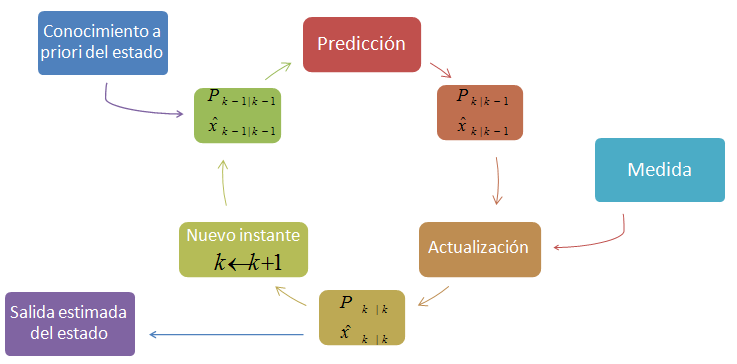
\includegraphics[width=.8\textwidth]{./pics_kalman/kal.png}
	\caption{Diagrama de flujo del filtro de Kalman}
	\label{fig:kal}
\end{figure}

Una vez que llega la siguiente medida de los sensores, contaminada necesariamente con ruido, las estimaciones son actualizadas en la etapa de \textbf{actualización}, mediante la utilización de un \emph{promedio ponderado}, dándole mayor peso a las estimaciones con menor incertidumbre en cada paso, obteniendo la estimación del estado para el instante k: $P_{k|k}$ y $\hat{x}_{k|k}$.\\

Por otro lado, las mayores restricciones que impone el filtro de Kalman son que el sistema dinámico subyacente debe ser lineal y que los ruidos presentes deben ser blancos y Gaussianos.\\

El sistema dinámico que queremos estimar, como se puede ver en el capítulo \ref{chap:modelo}, es claramente \textbf{no lineal}, por lo que se debe buscar alguna altenativa al filtro de Kalman clásico. Al investigar en la literatura existente, basados en \cite{bib:kalman} y \cite{bib:kalman2}, se decide implementar un filtro de Kalman extendido para la estimación del vector de estados.

\section{Filtro de Kalman Extendido (EKF)}

El filtro de \emph{Kalman extendido (EKF)} es la versión no lineal del filtro de Kalman. Linealiza en torno a una estimación de la media y la covarianza. En caso de conocer con exactitud el modelo de transición de estados, el EKF se considera el standard en la estimación no lineal de sistemas de navegación.\\

\subsection{Modelo matemático}

El sistema dinámico sigue el modelo:\\

$$\mathbf{x}_{k} = f(\mathbf{x}_{k-1}, \mathbf{u}_{k-1}) + \mathbf{w}_{k-1}$$

$$\mathbf{z}_{k} = h(\mathbf{x}_{k}) + \mathbf{v}_{k}$$

donde $\mathbf{w}_k$ y $\mathbf{v}_k$ son los ruidos de proceso y observación respectivamente. Se asume que son gaussianos y de media nula. Sus matrices de covarianza son $\mathbf{Q}_k$ y $\mathbf{R}_k$ respectivamente.

La función $f$ es utilizada para hallar el estado predicho a partir del estado previo, y de forma análoga la función $h$ se utiliza para hallar la medida predicha a partir del estado. Dicho de otro modo, la función $f$ guarda información sobre la evolución del estado, mientras que la función $h$ representa la transformación entre el vector de estados y la observación ideal (sin ruido). Dada la no linealidad del sistema, las funciones $f$ y $h$ no pueden ser aplicadas directamente a la covarianza. En su lugar se computa su \textbf{Jacobiano}, una matriz de derivadas parciales. Es importante destacar que el filtro de Kalman Extendido no tiene propiedades de optimalidad y su precisión dependerá en gran medida de la precisión de la linealización. Dado que se realiza una linealización dinámica, no hay manera de conocer su performance de antemano (por mayor detalles referirse a \cite{bib:kay}).\\
Para la predicción del estado se utilizan las ecuaciones del modelo físico del cuadricóptero presentadas en el capítulo \ref{chap:modelo}.\\

Las ecuaciones que gobiernan el comportamiento del filtro de Kalman Extendido son:
\begin{itemize}
	\item Predicción:
	\begin{itemize}
		\item Estimación de la predicción del estado
		$$\hat{\mathbf{x}}_{k|k-1} = f(\hat{\mathbf{x}}_{k-1|k-1}, u_{k-1})$$
		\item Estimación de la predicción de la covarianza
		$$ \mathbf{P}_{k|k-1} =  {{\mathbf{F}_{k-1}}} \mathbf{P}_{k-1|k-1}{  {\mathbf{F}_{k-1}^T}} + \mathbf{Q}_{k-1} $$		
	\end{itemize}
	\item Actualización
	\begin{itemize}
		\item Residuo de medida
		$$\tilde{\mathbf{y}}_{k} = \mathbf{z}_{k} - h(\hat{\mathbf{x}}_{k|k-1})$$
		\item Residuo de covarianza
		$$\mathbf{S}_{k} = { \mathbf{H}_{k}}\mathbf{P}_{k|k-1}{ \mathbf{H}_{k}^\top} + \mathbf{R}_{k}$$
		\item Ganancia de Kalman
		$$\mathbf{K}_{k} = \mathbf{P}_{k|k-1}{ \mathbf{H}_{k}^\top}\mathbf{S}_{k}^{-1} $$
		\item Estimación actualizada del estado
		$$\hat{\mathbf{x}}_{k|k} = \hat{\mathbf{x}}_{k|k-1} + \mathbf{K}_{k}\tilde{\mathbf{y}}_{k} $$
		\item Estimación actualizada de la covarianza.
		$$ \mathbf{P}_{k|k} = (I - \mathbf{K}_{k} { \mathbf{H}_{k}}) \mathbf{P}_{k|k-1} $$		
	\end{itemize}
\end{itemize}

Las matrices de transición de estados y observación son los siguientes jacobianos:
$$ { \mathbf{F}_{k-1}} = \left . \frac{\partial f}{\partial \mathbf{x} } \right \vert _{\hat{\mathbf{x}}_{k-1|k-1},\mathbf{u}_{k-1}} $$
\vspace{10pt}
$$ { \mathbf{H}_{k}} = \left . \frac{\partial h}{\partial \mathbf{x} } \right \vert _{\hat{\mathbf{x}}_{k|k-1}} $$


\subsection{Esquema general del estimador de estados}

Los datos (en algunos casos redundantes) obtenidos de los diferentes sensores son combinados usando un filtro de Kalman Extendido para determinar el vector de estados, detallado en \ref{chap:modelo}:
\begin{equation}
  \label{eq:estado}
  X=\left\lbrace  x,y,z, \theta,\varphi,\psi, v_{q_z},v_{q_y},v_{q_z},\omega_{q_x},\omega_{q_y},\omega_{q_z} \right\rbrace
\end{equation}

De la caracterización de los motores, capítulo \ref{chap:motores}, se obtiene la relación matemática entre la fuerza realizada por cada uno de los motores contra la velocidad de giro del mismo y la relación entre la el torque de \emph{drag} realizado por cada motor y su velocidad de giro. Por lo tanto basta con controlar la velocidad de giro de los motores para poder determinar todas las entradas al sistema. Se considerará entonces como entrada al sistema las velocidades angulares $w_1$, $w_2$, $w_3$, $w_4$ de los 4 motores.\\

El esquema general del integración de los sensores se puede ver en la figura \ref{fig:diagrama_kalman}, el cual se pasa a describir a continuación.

\begin{figure}[h!]
	\centering
	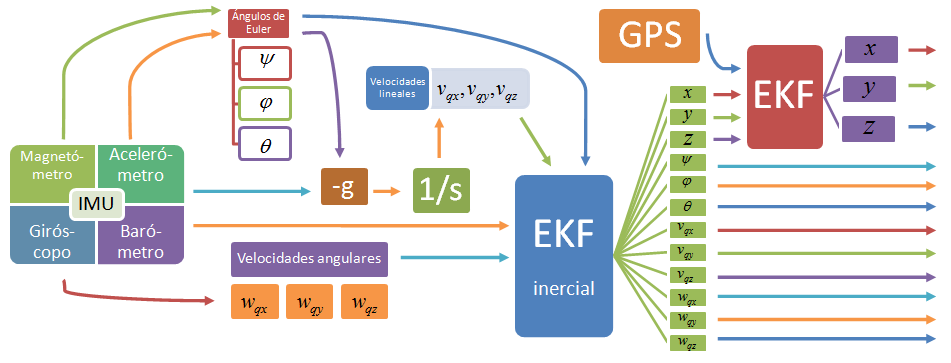
\includegraphics[width=1\textwidth]{./pics_kalman/diagrama_kalman.png}
	\caption{Esquema general de integración de sensores}
	\label{fig:diagrama_kalman}
\end{figure}

Básicamente se utilizan 2 filtros de Kalman distintos.\\
El primero (Kalman inercial) se encarga de estimar los 12 estados del vector $X$ considerando solamente las medidas obtenidas del sensor inercial (\textbf{IMU}). Para la estimación de los ángulos se utiliza una combinación entre las medidas obtenidas del acelerómetro y del magnetómetro, para la estimación de las velocidades angulares se utiliza directamente la medida arrojada por el giróscopo y para las velocidades lineales se trabaja con las medidas arrojadas por el acelerómetro. A su vez, al estar considerado el modelo físico dentro del filtro, se utilizan las estimaciones de todas las variables para determinar las predicciones del resto. Para la estimación de la posición en ``x'' y en ``y'' no se tiene ninguna medida de corrección, por lo que quedará determinado únicamente por la predicción del modelo físico, lo cual resulta en una acumulación significativo de error.
El segundo se encarga de la integración entre la salida del primero y los datos recogidos por el GPS. En este caso se tiene medida de corrección para la posición en todas las direcciones, resolviendo el problema de acumulación de error del filtro inercial.


La separación en 2 filtros distintos otorga una interesante flexibilidad. Es posible utilizar una estimación del estado estando a puertas cerradas, sin la necesidad de señal de GPS, a costas de una peor estimación de las posiciones y velocidades lineales en ``x'' e ``y''.

\subsubsection*{Orientación}

En estado estático, los ángulos de \emph{pitch} y \emph{roll} pueden ser determinados proyectando el vector medido de aceleración gravitacional por el acelerómetro. A su vez, los cambios entre el sensor magnético y el vector geomagnético medido, representan al ángulo \emph{yaw}. Por lo tanto, el conjunto del acelerómetro y magnetómetro son capaces de determinar la orientación del cuadricóptero mediante las medidas del vector de aceleración gravitatoria y el vector geomagnético. Dado que el magnetómetro digital no introduce acumulación de error, este sistema ha sido muy utilizado para la determinación estática de la posición, como se puede ver en \cite{bib:euler_magneto_acc}.

%TODO nunca va a haber otra aceleracion que no sea en z, por la dinámica del quad? entonces el razonamiento anterior no solo vale para estado estatico.

\subsubsection{Aceleración}

Para poder obtener la transformación entre el vector de estados y la observación es necesario entender qué aceleración medirá el acelerómetro. Como se explica en \ref{acelerometro}, dicho dispositivo referencia su medida a un sistema en caída libre, por lo que por ejemplo al estar quieto se deberá medir la aceleración gravitatoria ($g$).\\
Como se puede ver en el esquema mostrado en la figura \ref{fig:diagrama_kalman}, el acelerómetro es utilizado para estimar las variables de estado $v_{qx}$, $v_{qy}$ y $v_{qz}$, correspondientes a las velocidades lineales medidas en el sistema del cuadricóptero. No se debe confundir la derivada de estas variables con la aceleración medida por el acelerómetro. Por un lado se debe realizar el pasaje del sistema de referencia del cuadricóptero hasta un sistema de referencia inercial fijo en el mundo, y por otro lado se debe tener en cuenta el pasaje de este último hasta el sistema de referencia del acelerómtro (el sistema en caída libre), por ello es que se incluye el bloque ``-g'' en el diagrama de la figura \ref{fig:diagrama_kalman}.

% TODO hablar de Q y R. capaz poner 2 ejemplos de lo mismo q den bien distinto


\section{Resultados}

%\begin{figure}[h!]
%	\centering
%	\includegraphics[width=0.2\textwidth]{./pics_kalman/}
%	\caption{Canmore GT-730F}
%	\label{fig:gps}
%\end{figure}



\end{document}